\documentclass[a4paper, 12pt]{article}
\usepackage[T2A]{fontenc}
\usepackage[english, russian]{babel}
\usepackage{graphicx}
\graphicspath{{./Images/}}
\usepackage[utf8]{inputenc}
\usepackage{alltt}
\usepackage[
backend=biber,
style=alphabetic,
sorting=ynt
]{biblatex}
\addbibresource{sample.bib}
\usepackage{listings}


\title{Аппаратные средства вычислительной техники - параллельные вычисления на CUDA ядрах}
\author{Vladislav Khvan & Khvan Vladislav}
\date{June 2023}

\begin{document}

\maketitle % делаем титульный лист документа

\newpage

\section{Что такое CUDA-ядра?}
\textit{Ядро CUDA, потоковый процессор, блок шейдеров} - все это синонимы вычислительного блока GPU, который выполняет расчет данных. NVIDIA по традиции называет их ядрами CUDA, где CUDA расшифровывается как Compute Unified Device Architecture. Ядра CUDA отличаются от ядер процессора, они намного менее сложные и имеют высокую степень специализации под обрабатываемые данные
    \begin{figure}[h]
        \centering
        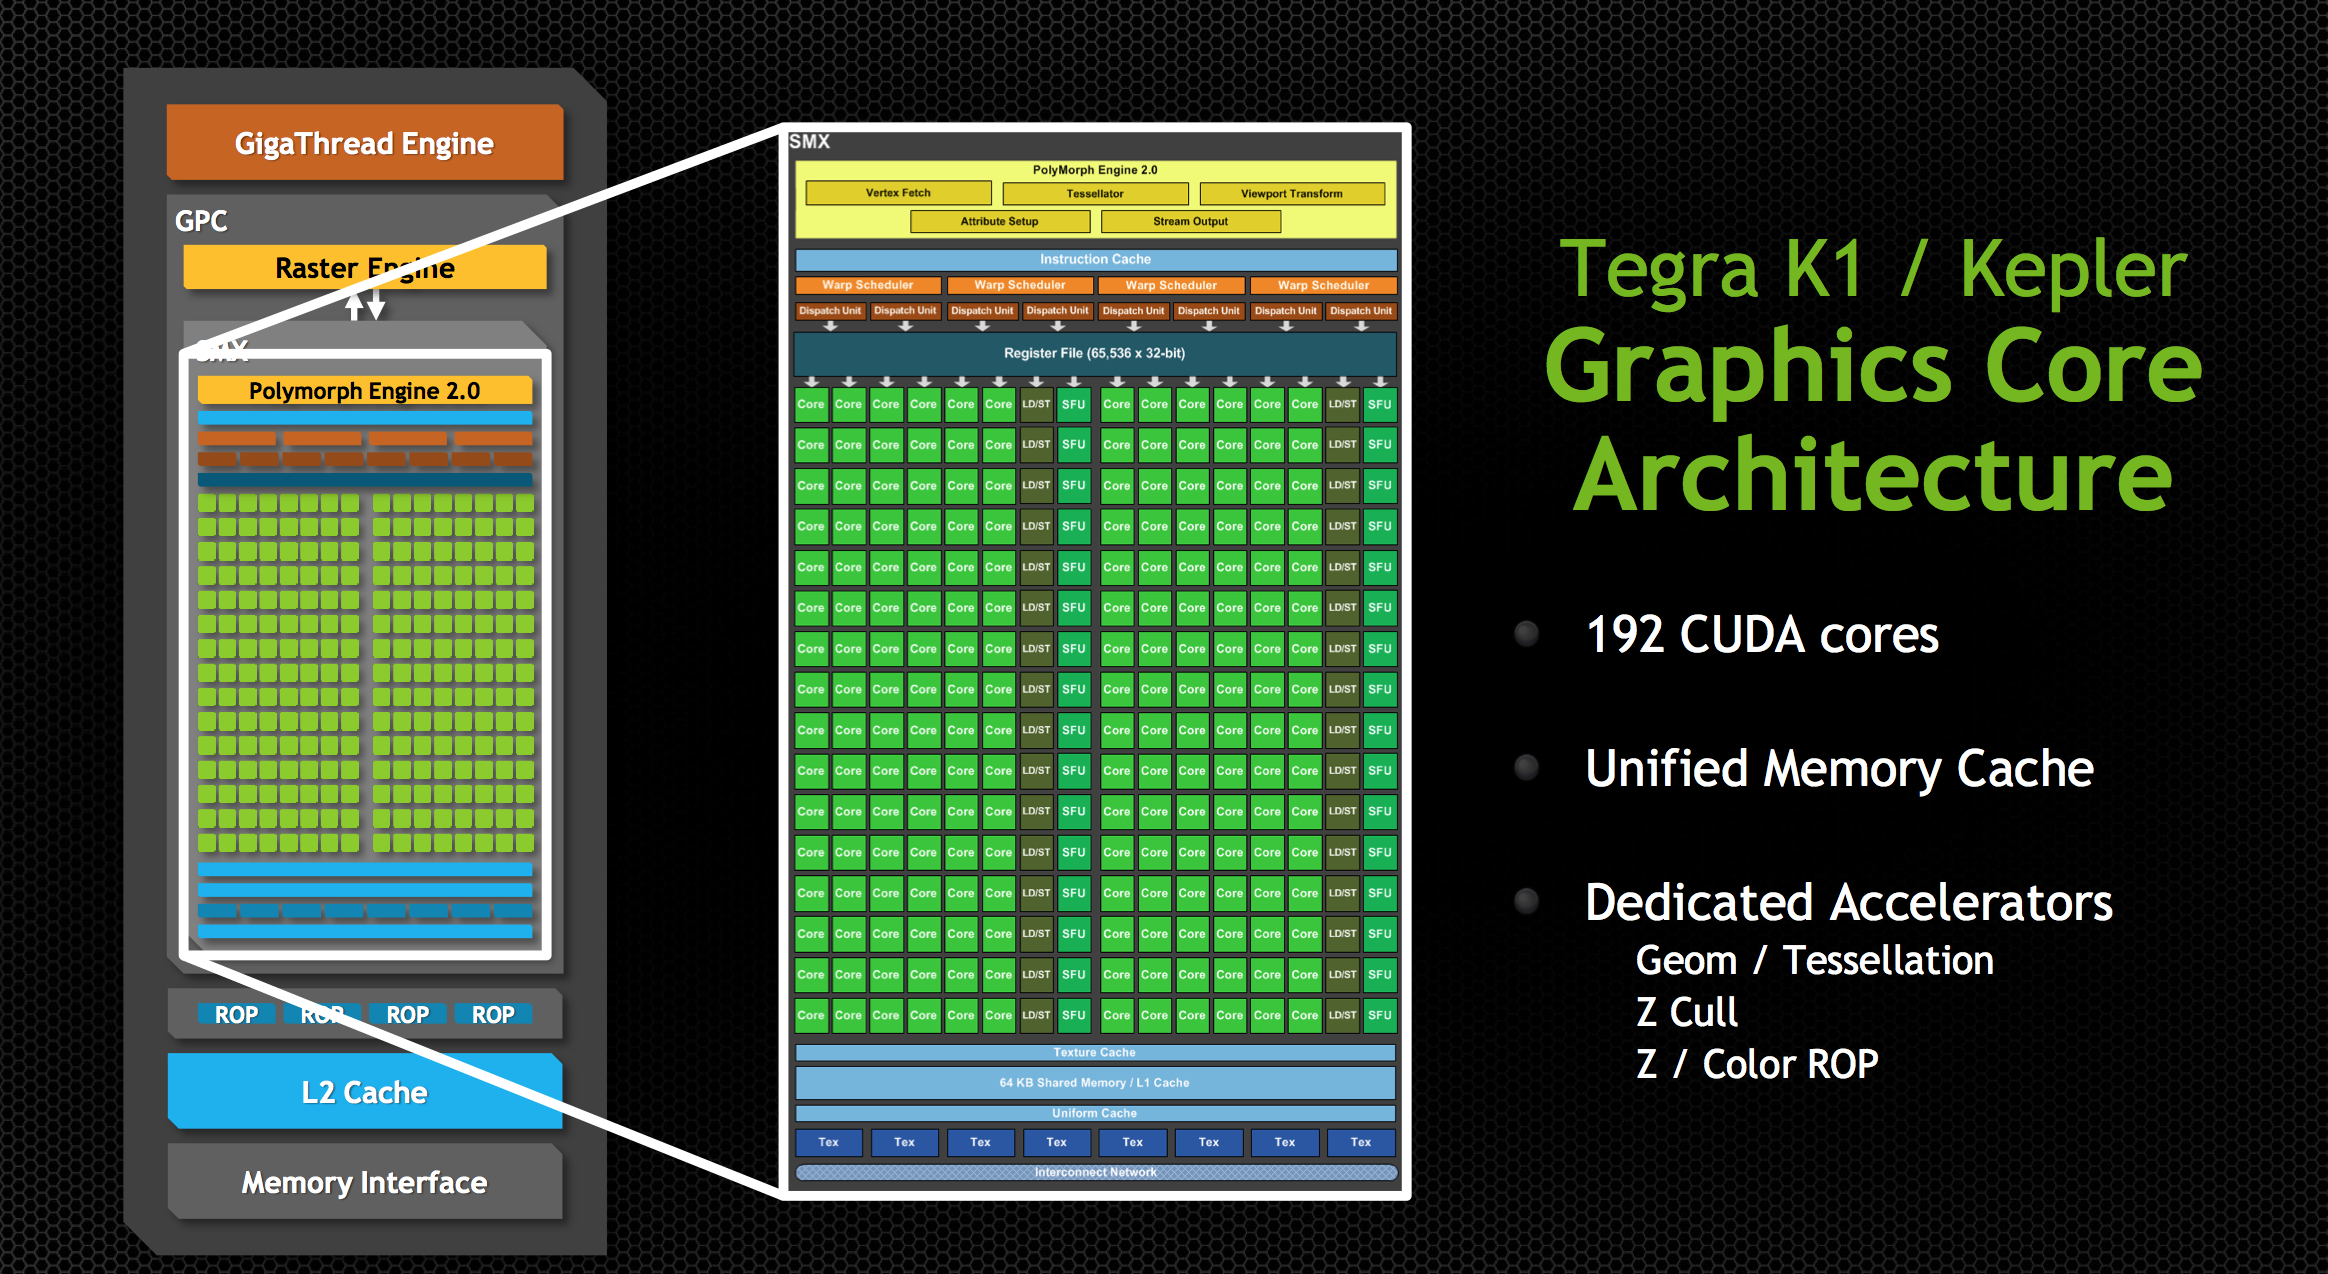
\includegraphics[width=\textwidth]{CUDA-previev.png}
        \caption{Представление CUDA-ядер}
        \label{fig:CUDA-previev}
    \end{figure}

\section{Где используются CUDA-ядра?}

CUDA-ядра (Compute Unified Device Architecture) - это ядра, которые используются для выполнения параллельных вычислений на графических процессорах (ГПУ) с архитектурой NVIDIA. Они представляют собой специально оптимизированный набор инструкций и программного обеспечения, которые позволяют программистам разрабатывать и выполнять высокопроизводительные параллельные приложения на ГПУ.

Вот некоторые основные причины использования CUDA-ядер:
\begin{enumerate}
    \item Ускорение вычислений: CUDA позволяет использовать параллельные вычисления на ГПУ, которые обладают большим количеством ядер и параллельной обработкой потоков данных. Это особенно полезно для приложений, требующих высокой производительности, таких как научные вычисления, обработка изображений, машинное обучение и глубокое обучение.
    \item Распределение работы: CUDA позволяет эффективно распределить задачи между множеством ядер ГПУ. Каждое ядро может выполнять свою часть работы независимо, что увеличивает общую скорость обработки данных.
    \item Параллельная обработка данных: CUDA позволяет одновременно обрабатывать большие объемы данных, разделяя их между множеством ядер ГПУ. Это особенно полезно для задач, таких как обработка изображений, видео и аудио, где необходимо быстро обрабатывать большие объемы информации.
    \item Ускорение машинного обучения: Графические процессоры, поддерживаемые CUDA, могут быть использованы для ускорения обучения и выполнения моделей машинного обучения и глубокого обучения. CUDA предоставляет оптимизированные библиотеки и инструменты, такие как cuDNN (CUDA Deep Neural Network library), которые значительно увеличивают производительность в задачах обработки данных и тренировке нейронных сетей.
    \item Переносимость: CUDA-ядра могут быть использованы на различных платформах с поддержкой NVIDIA GPU, что обеспечивает переносимость параллельных вычислений между различными системами.

\end{enumerate}

\section{Что нужно уметь для программирования на CUDA-ядрах?}
Ну для начала Вы должны уметь вывести "Hello World!" на С++

\begin{lstlisting}
#include <iostream>

int main() {
    std::cout << "Hello World!" << std::endl;
    return 0;
}
\end{lstlisting}

Также нужно знать некоторые программные библиотеки, базовые концепции параллельных вычислений и понимание архитектуры CUDA-ядер.

\section{В чём плюсы параллельного вычисления?}
Параллельное вычисление позволяет быстрее и эффективнее выполнить определённые операции, что логично.

$S=T_1/T_n$
\begin{verbatim}
Где:
S - Ускорение параллельной программы
T_1 - Время выполнения последовательной программы
T_n - Время выполнения параллельной программы на n потоках
\end{verbatim}

\begin{center}
\begin{tabular}{||c c||} 
     \hline
     Количество потоков & Время выполнения программы \\ [0.5ex] 
     \hline\hline
     1 & 32 с.\\ 
     \hline
     2 & 16 с.\\
     \hline
     4 & 8 с. \\
     \hline
     8 & 4 с\\
     \hline
\end{tabular}
\end{center}

\begin{thebibliography}{2}
    \bibitem{first_bib}
     Боресков А.В., Харламов А.А. - Основы работы с технологией CUDA - (2010 )
     \bibitem{second_bib}
     Сандерс Дж., Кэндрот Д. - Технология CUDA в примерах - (2011)
\end{thebibliography}

\end{document}
